% CREATED  14 May 2015
% MODIFIED 29 May 2015
% PURPOSE present to a group of statisticians from the public health faculty at Herston

\documentclass[xcolor=svgnames,aspectratio=169]{beamer} 

\setbeamercolor{normal text}{bg=white,fg=black} 
\usecolortheme[named=blue]{structure} 
\usetheme{default} 

\usepackage{graphicx}
\usepackage{subfigure}
%\usepackage[space]{grffile}
\usepackage{rotating}
\usepackage{booktabs}
\usepackage{amsmath}
\usepackage{multicol}
\usepackage{multirow}
\usepackage{natbib}
\usepackage{bibentry}

\def\Tiny{\fontsize{1pt}{1pt}\selectfont}

\setbeamersize{text margin left=0.2em} % used to allow wide tables to fit-in a slide

\begin{document}

\title{Hazard function models \\ a new tool to estimate fish mortality rates from age data}
\subtitle{with application to Qld mullet ({\it Mugil cephalus})}

\author{Marco Kienzle}
\institute{Qld Department of Agriculture, Fisheries - Dutton Park\\ UQ's school of Agriculture and Food Sciences - St Lucia}
\date{\today} 

%%%%%%%%%%%%%%%%%%%%%%%%%%%%%%
\frame{\titlepage}

%% %%%%%%%%%%%%%%%%%%%%%%%%%%%%%%
\frame{\frametitle{Contributions acknowledgements}

The development of this method, presentation and paper is the result of many discussions and inputs from a range of people (in no particular order) \\
\vspace{0.25cm}

C. Millar (FRS-Scotland), W.N. Venables (CSIRO), N. White (QUT), P. Baker and R. Ware (UQ-School of Public Health), D. Mayer and J. McGilvray (DAF), 4 anonymous reviewers \\
\vspace{0.5cm}

Some publications about survival analysis: \\
\vspace{0.25cm}

Cox, D.R. and Oakes, D. (1984) {\bf Analysis of survival data}, {\it Chapman and Hall Ltd, London} \\

Kleinbaum, D.G. and Klein, M. (2005) {\bf Survival Analysis: A Self-Learning Text} {\it Springer, New York}\\

Ferrandis, E. and Hern\'{a}ndez, P. (2007) {\bf Direct Survival Analysis: a new stock assessment method} {\it Scientia Marina}, 71:1 \\
}

%% \begin{itemize}
%% \item governments are interested in sustainable exploitation of their natural resources
%% \item fishermen and research organizations collect data to assess the status of fish species
%% \item a mathematical model is calibrated to available data and later used to determine sustainable levels of fishing
%% \item Essentially, a stock assessment model estimates mortality rates (and recruitment)
%% \end{itemize}

%% \vspace{0.5cm}
%% Motivations for doing this work \\
%% \begin{itemize}
%% \item provide estimates of fish mortality rates using age data from a sample of catch
%% \item work within the likelihood framework in order to compare different models
%% \end{itemize}

%%%%%%%%%%%%%%%%%%%%%%%%%%%%%%%%%%%
\frame{\frametitle{Motivations for this collaboration between biometry and LTMP}

\begin{itemize}
\item convert LTMP data into useful scientific information for fisheries managers
\item apply statistical methods to estimate mortality rates from age data
\item choose methods capable of updating mortality estimates yearly as new data become available
\end{itemize}
}
%%%%%%%%%%%%%%%%%%%%%%%%%%%%%%%%%%%
\frame{\frametitle{Methods applied to perform this work}

\begin{itemize}
\item critical evaluation of available methods to estimate mortality rates (a4a, CASAL, SS3, etc...)
\item determine the accuracy and precision of each method using Monte Carlo simulations (quality control, testing)
\item comparison of statistical methods using the likelihood approach (R.A. Fisher) and selection of the maximum likelihood mortality rates estimates %only two methods available for comparison to date (looking for more)
%\item apply likelihood approach to compare ideas, hypotheses (multiplicity of models) 
\end{itemize}

"... it will be found that the method here outlined is illuminating in all similar cases when the same quantity may be ascertained by more than one statistical formula" (R.A. Fisher introducing the likelihood method in 1920)
}

%% %%%%%%%%%%%%%%%%%%%%%%%%%%%%%%
\frame{\frametitle{The problem of estimating mortality rates in the age-structure context}


Estimate natural and fishing mortality rates for all ages and years from age data\\

For example,

\[
\begin{array}{cc|ccccccc}
& & \multicolumn{7}{c}{ \rm{age-groups} } \\
& & 1  & 2 & 3    & \ldots & j & \ldots & n \\ \hline 
& 1 & 0.3 & 0.35 & 0.4 & \ldots & \ldots & & \ldots \\
& \vdots &  \vdots & \vdots & \ldots  & & \ldots & & \ldots \\
\multirow{3}{*}{\begin{sideways} years \end{sideways}} & & & & & & \\
& i & \vdots & \vdots & 0.65  & & M_{i,j} + F_{i,j} & & \ldots \\
& \vdots & & &  0.7  & & \ldots & & 0.8 \\
& p & &  & \dots  & & 0.8 & & 0.9 \\
\end{array}
\]


}

%% %%%%%%%%%%%%%%%%%%%%%%%%%%%%%%
\frame{\frametitle{Mullet age data from the long term monitoring program (LTMP)}

\begin{figure}[!h]
     \centering
      \includegraphics[scale=0.35,angle=-90]{Graphics/MulletNbAtAge.ps}
\end{figure}

3-5 years old mullet were most frequent in the sample

}

%%%%%%%%%%%%%%%%%%%%%%%%%%%%%%
\frame{\frametitle{Deterministic theory for fishing a single cohort} 

%\begin{itemize}
Exponential decline a \textcolor{red}{cohort} through time from \cite{quin99b}
\begin{equation}
\frac{dN}{dt} = - F N - M N
\end{equation}

\begin{equation}
N(t) = N_{0} e^{-(F+M) t}
\end{equation}

%\begin{itemize}
Baranov catch equation (1910)
\begin{equation}
\frac{dC}{dt} = F N
\end{equation}

\begin{equation}
C_{0 \rightarrow \tau} = \frac{F}{M+F} N_{0} (1 - e^{-(M+F) \tau})
\end{equation}

%Deterministic parameters estimations ($N_{0}, M, F$) by least square or likelihood using catches at age \\
%{\color{red} PROBLEMS}: high number of parameters, convergence failure, require accurate starting values, fixing some parameters as a solution, etc...
}

%%%%%%%%%%%%%%%%%%%%%%%%%%%%%%
\frame{\frametitle{Cross sectional approach to estimate total mortality (M+F) for mullet}

\begin{figure}[!h]
     \centering
      \includegraphics[scale=0.35,angle=-90]{Graphics/MulletCrossSectionalAnalysis4Presentation.ps}
\end{figure}

}
%%%%%%%%%%%%%%%%%%%%%%%%%%%%%%
\frame{\frametitle{Monte Carlo simulations to test statistical methods}

\begin{itemize}
  \item Validate methods and their computer implementations (regression tests, software eng.)
  \item Quantify statistical properties of methods (bias, variance, sentitivity, ...)
  \item Compare alternative methods (in stock assessment: National Research Council (1999) Improving Fish Stock Assessments, National Academic Press.)
  \item Simulated 8000 age sample with parameters consistent with sea mullet fishery (0 $\leq$ age $\leq$ 16 years)
\end{itemize}


\begin{table}[ht]
\centering
\begin{tabular}{lll}
  \hline
Variable type & Distribution & Parameters \\
  \hline
recruitment               & uniform & min=4e6, max=8e6   \\
natural mortality         & uniform & min=0.30, max=0.36 \\
catchability              & uniform & min=1.5e-4, max=2.5e-4 \\
fishing effort            & uniform & min=2e3, max=4e3   \\
gear selectivity $\alpha$ & uniform & min=7.5, max=8.5      \\
gear selectivity $\beta$  & uniform & min=2, max=3       \\
   \hline
\end{tabular}
\end{table}

}


%%%%%%%%%%%%%%%%%%%%%%%%%%%%%%
\frame{\frametitle{Monte Carlo simulations: \\ cross sectional provides inaccurate estimates of mortality}

\begin{figure}[!h]
     \centering
      \includegraphics[scale=0.35,angle=-90]{Results/Graphics/MCtestCrossSectional4Presentation.ps}
\end{figure}
}

%% %%%%%%%%%%%%%%%%%%%%%%%%%%%%%%
\frame{\frametitle{Shortcomings of cross sectional analysis}

\begin{itemize}
 \item provides an inaccurate estimate of total mortality
 \item ignores the fact that catches are made of several cohorts
 \item it mixes recruitment and mortality signals into a noisy estimator
 \item uses only a subset of the data (48/88=54\% in the case of mullet)
 \item it doesn't offer a framework where we can compare different ideas (take it or leave it)
\end{itemize}

}

%% %%%%%%%%%%%%%%%%%%%%%%%%%%%%%%
\frame{\frametitle{Survival analysis: a probabilistic theory for fishing a single cohort}

Survival analysis \citep{cox84b, scimar42} using a constant hazard function

\begin{equation}
h(t; \theta) = M + F
\end{equation}

The probability density function (pdf)

\begin{equation}
f(t; \theta) = (M + F) \ e^{-(M+F)t} = M \ e^{-(M+F)t} + F \ e^{-(M+F)t}
\end{equation}

The likelihood \citep{edwards1992likelihood} of a sample of fish caught in the fishery ($S_{i}$) using the probability of dying in the interval $[a_{i}; a_{i+1}]$.

\begin{equation}
\mathcal{L}  = \prod_{i=1}^{n} \bigl ( \int_{t=a_{i}}^{t=a_{i+1}} f(t; \theta) \ dt \bigr ) ^ {S_{i}} 
\end{equation}

The logarithm of the likelihood
\begin{equation}
{\rm log}(\mathcal{L}) = \sum_{i=1}^{n} S_{i} \ {\rm log} \bigl ( e^{-(M+F) \times a_{i}} - e^{-(M+F) \times a_{i+1}} \bigr )
\end{equation}

}

%%%%%%%%%%%%%%%%%%%%%%%%%%%%%%%%%
\frame{\frametitle{Illustration of survival analysis concepts}

\begin{figure}[!h]
     \centering
      \includegraphics[scale=0.35,angle=-90]{Results/Graphics/IllustrationOfSurivalAnalysisConcepts.ps}
\end{figure}
}
%%%%%%%%%%%%%%%%%%%%%%%%%%%%%%%%%
\frame{\frametitle{Hazard models for more complicate situations}

Fishing mortality is a function of effort (E)\\
$F(t) = q \ E(t)$ $\rightarrow h(t; \theta) = M + q \ E(t)$\\

\vspace{0.5cm}

Gear selectivity (s) varies with age\\
$F(t) = q \ s(t) \ E(t)$ $\rightarrow h(t; \theta) = M + q \ s(t) \ E(t)$\\

%% \begin{figure}[!h]
%%      \centering
%%       \includegraphics[scale=0.25,angle=-90]{../Herston2015/Graphics/LogisticGearSelectivity.ps}
%%     \end{figure}

}

%%%%%%%%%%%%%%%%%%%%%%%%%%%%%%%%%
\frame{\frametitle{Survival analysis is a flexible method to analyze age data}

\begin{itemize}
\item restricted range of ages $\rightarrow$ truncated pdf
\item +group $\rightarrow$ integrate over a larger interval $ [a_{+}; \infty[ $
\end{itemize}
}


%%%%%%%%%%%%%%%%%%%%%%%%%%%%%%%%
\frame{\frametitle{Applying hazard model to data from multiple cohort}

\[
\begin{array}{cc|ccccc}
& & \multicolumn{5}{c}{ \rm{age-groups} } \\
& & 1      & \ldots & j & \ldots & n \\ \hline 
& 1 & \ldots  & & \ldots & & \ldots \\
& \vdots &  \ldots  & & \ldots & & \ldots \\
\multirow{3}{*}{\begin{sideways} years \end{sideways}} & & & & & & \\
& i & \dots  & & S_{i,j} & & \ldots \\
& \vdots &  \ldots  & & \ldots & & \ldots \\
& p & \dots  & & \ldots & & \ldots \\
\end{array}
\]

\begin{itemize}
 \item $n + p - 1$ cohorts, separability $F_{i,j} = q \ E_{i} \otimes s_{j}$
\end{itemize}

The likelihood
\begin{equation}
\mathcal{L} = \prod_{k=1}^{n+p-1} \prod_{l=1}^{r_{k}}  \bigl ( \int_{t=a_{k,l}}^{t=a_{k,l+1}} g_{k}(t; \theta) \ dt \bigr ) ^ {S_{k,l}}
\end{equation}

}

%%%%%%%%%%%%%%%%%%%%%%%%%%%%%%
\frame{\frametitle{Computer implementation of these methods}

Methods implemented in R \citep{R} in a package called Survival Analysis for Fisheries Research (SAFR) \\

\vspace{0.5cm}

Available at: \url{https://github.com/mkienzle/SurvivalAnalysisForFisheries} \\

\vspace{0.5cm}

Manuscript was published after a double blind reviewing process: \\

Kienzle, M. (2015) {\bf Hazard Function Models to Estimate Mortality Rates Affecting Fish Populations with Application to the Sea Mullet (Mugil cephalus) Fishery on the Queensland Coast (Australia)} {\it Journal of Agricultural, Biological, and Environmental Statistics}, 21(1), p. 76--91, doi:10.1007/s13253-015-0237-y \\ 
 
\vspace{0.5cm}

One of the reviewer's comment was : "The manuscript is well written and statistically sound."
%: \url{http://dx.doi.org/10.1007/s13253-015-0237-y}

 
}

%% %%%%%%%%%%%%%%%%%%%%%%%%%%%%%%
%% \frame{\frametitle{Testing hazard functions with Monte Carlo simulations}

%% Simulate a fishery using random population characteristics (recruitment, natural mortality) and random catch (catchability, effort and gear selectivity)\\

%% \vspace{0.5cm}

%% 2 types of sampling to generate artificial catch data
%% \begin{itemize}
%% \item random sampling (benchmark) [strategy 1]
%% \item systematic [strategy 2] (weighted by catch or un-weighted)
%% \end{itemize}
 
%% }

%%%%%%%%%%%%%%%%%%%%%%%%%%%%%%
\frame{\frametitle{Survival analysis provides accurate estimates of mortality}

\begin{figure}[!h]
     \centering
      \includegraphics[scale=0.35,angle=-90]{Results/Graphics/MCtestSurvivalAnalysis4Presentation.ps}
\end{figure}
}

%% %%%%%%%%%%%%%%%%%%%%%%%%%%%%%%
%% \frame{\frametitle{Hazard function models can estimate natural mortality \\when age-sample are weighted by total catch}

%% \begin{figure}[!h]
%%      \centering
%%       \includegraphics[scale=0.35,angle=-90]{../../Results/Graphics/Estimating-NaturalMortality4Presentation.ps}
%%     \end{figure}

%% }
%% %%%%%%%%%%%%%%%%%%%%%%%%%%%%%%
%% \frame{\frametitle{Sampling strategy 2 using weighted samples can estimate catchability (q)}

%% \begin{figure}[!h]
%%      \centering
%%       \includegraphics[scale=0.35,angle=-90]{../../Results/Graphics/Estimating-Catchability4Presentation.ps}
%%     \end{figure}

%% }

%% %%%%%%%%%%%%%%%%%%%%%%%%%%%%%%
%% \frame{\frametitle{Hazard function fit better than the traditional multinomial approach}

%% \begin{figure}[!h]
%%      \centering
%%       \includegraphics[scale=0.35,angle=-90]{../../Results/Graphics/ComparisonOfNegLL4Presentation.ps}
%%     \end{figure}

%% }
%%%%%%%%%%%%%%%%%%%%%%%%%%%%%%
\frame{\frametitle{Survival analysis is more precise than cross sectional analysis}

\begin{figure}[!h]
     \centering
      \includegraphics[scale=0.35,angle=-90]{Results/Graphics/ComparisonBetweenCSandSAmctestScatterPlot4Presentation.ps}
\end{figure}
}

%%%%%%%%%%%%%%%%%%%%%%%%%%%%%%
\frame{\frametitle{Survival analysis provides a model of all data}

\begin{figure}[!h]
     \centering
      \includegraphics[scale=0.35, angle = -90]{Graphics/ComparisonOfFitBetweenCSAndSA.ps}
\end{figure}
}

%%%%%%%%%%%%%%%%%%%%%%%%%%%%%%
\frame{\frametitle{Summary of methods comparison: \\cross sectional is less accurate at estimating mortality rates}

\vspace{0.5cm}
\begin{table}
\begin{center}

\begin{tabular}{|l | c | c|}
\hline
Characteristics        & Cross sectional & Survival analysis \\
\hline \hline
accuracy               & less        & more               \\
precision              & less        & more               \\
deals with cohorts     & no          & yes                \\
use all data           & no          & yes               \\
likelihood based       & no          & yes               \\
tested with MC         & yes         & yes               \\
estimate nat. mort.    & no          & yes               \\
-log($\mathcal{L}$)    & \textcolor{red}{22148.44}    & 18795.28          \\
\hline
\end{tabular}
\end{center}
\end{table} 
}

%%%%%%%%%%%%%%%%%%%%%%%%%%%%%
\frame{\frametitle{Qld mullet fishery mortality rates estimates}% (estimated with survival analysis) \\ have been trending down over the last 8 years}

\begin{figure}[!h]
     \centering
      \includegraphics[width=0.25\textwidth,scale=0.25, angle = -90]{Results/Graphics/Model2-EstimatedTrendsInMortality.ps}
      \includegraphics[width=0.25\textwidth,scale=0.25, angle = -90]{Results/Graphics/CrossSectional-EstimatedTrendsInMortality.ps}\\
      \includegraphics[width=0.25\textwidth,scale=0.25, angle = -90]{Results/Graphics/TrendInFishinEffort.ps}
\end{figure}
}

%%%%%%%%%%%%%%%%%%%%%%%%%%%%%%
\frame{\frametitle{Conclusions}

\begin{itemize}
  \item There exists an accurate and more precise method to estimate mortality rates from LTMP age data than currently used in DAF
\item Survival analysis
  \begin{itemize}
    \item is fast, robust, provides accurate estimates of mortality on a yearly basis
    \item is published \citep{Kienzle2015, scimar42, cox84b}% but not applied in DAF (yet !) might require some time for adoption (if at all)
    \item is operational to analyze DAF's mullet data 
    \item is more precise than cross sectional analysis 
    \item is a general age-structured method for stock assessment applicable to other stocks
%    \item does not deal with incomplete effort time series (yet!) (recreational fisheries)
%    \item requires advanced skills in statistics to develop models and troubleshoot the analyses
  \end{itemize}
\end{itemize}

\nobibliography{/home/mkienzle/mystuff/Bibliography/a-JLong,/home/mkienzle/mystuff/Bibliography/Biblio}
\bibliographystyle{plainnat}

}

%% %%%%%%%%%%%%%%%%%%%%%%%%%%%%%%
\frame{\frametitle{Thank you for your attention}

\begin{itemize}
 \item We value your feedback
% \item Do you know of any R package readily available to process fish-age data ?
% \item Would you like to contribute your expertise to articles on this topic ?
\end{itemize}

%% \nobibliography{/home/mkienzle/mystuff/Bibliography/a-JLong,/home/mkienzle/mystuff/Bibliography/Biblio}
%% \bibliographystyle{plainnat}

}


\end{document}
